\documentclass{article}
\usepackage{graphicx}
\usepackage[left=4cm,right=4cm,top=2cm,bottom=2cm]{geometry}
\usepackage{pgfplots}

\begin{document}

\title{Sentiment Classification}
\author{Devaux Matthieu}


\maketitle

\begin{abstract}
Foresee the smiley of a twitter message
\end{abstract}

\section{Introduction}

The aim of this project is to create a program that can foresee what smiley would be at the end of a tweet. I searched different way to make this possible and that is what you will read about on this paper.


\section{Base}

I will present the base algorithm and code that I have use to create the sentiment classifier :\\
First we need to create a dictionary of the words that compose tweets with a happy face smiley and the ones with a sad face smiley. To do that we need to take the test file given for and classify them as happy word or sad word, but we need to differentiate the words that are specific to a sentiment or word that are commonly use in the two cases, in that optic I created a dictionary using dict(), I iterate all the phrases of the test set and each time a word is in a phrase with a sad smiley I decrement its value by one in the dictionary and each time it is in a phrase with an happy smiley I increment it by one. That way the value is positive if it is a used for the happy phrases, negative if it used for the sad phrase and it is zero if it is not used or used in both happy and sad phrases. \\
Now we need to take out from the dictionary all the word that would be to close to zero (meaning all the non-specific word), so we choose a threshold and all word whose absolute values of the number of iteration of the word is lower than the threshold is delete from the dictionary.\\
Finally, we should try to find the good smiley for some test twitter message, so what we do is use the dictionary and we compare in every tweet the word that are in our dictionary in the sad and happy messages, and with this result we try to figure the smiley. If the smiley is unknown we choose to return 0.

\subsection{How to compare the dictionary and the tweet}

Once we have decided what to compare, we have to choose how we are going to decide how to compare them. I have found two method :\\ one is to give to every world a value that is : \[ number\ of\ time\ that\ a\ word\ is\ found\ in\ positive\ tweets\ - number\ of\ time\ it\ is\ found\ in\ the\ positive\ tweets \]
in the training sets and then for each tweets we work on we give a value which is the sum of the dictionary value of all the word that are in the tweet and in the end if the results is positive we consider it is a happy smiley and if it is negative we consider it is a sad smiley (if it is zero we consider it unknown). \\
The other method is for each tweet to look at all the word that have positive value in the dictionary (that are more found in positive tweets) and compare to the number of word that have negative value (that are more found in negative tweets). If there is more positive word we say that the tweets has a happy face and if there is more negative word we say the tweets have a sad face (if there is the same amount on both side we say it is unknown).\\
So we are going to test both to see which one is the best :
\\
 \\
 test 1 :\\
 training set : little training set\\
 threshold to keep a word in the dictionary : 10\\
 way of comparing word : valueWordValue (the first way proposed )\\
 result : 0.6302\\
  \\
  \\
  test 2 :\\ 
 training set : little training set\\
 threshold : 10\\
 way of comparing word : valueWordNumber (the second way proposed )\\
 result :  0.66800\\
 \\
We can see that the second way is better than the first one so we are going to use valueWordNumber to compare word in the tweets.\\
 \\
I have created a third option that use both of those method : for each word it gets the sum of the value of positive words, the number of the positive words, the inverse of the sum of the value of the negative words (we inverse it so that it is positive) and the number of negative word and :\\
if the number or the value of the positive words is null then return -1\\
if the number or the value of the negative words is null then return 1\\
if both are null return an arbitrarily value (here I choose 1)\\
if  the results from valueWordValue and valueWordNumber created by those value are equal then return the value given by valueWordValue\\
if they are different then we compare the ratio of positive and negative of the value and the numbers and the one that is bigger is used as a method to return the results.\\
(the implementation is in util in the method valueWordMixValueNumber)\\
So now we test this method :\\
 \\
 test 3 :\\ 
 training set : little training set\\
 threshold : 10\\
 way of comparing word : valueWordMixValueNumber\\
 result :  0.65440\\
 \\

The value is still smaller so for now we are going to use valueWordNumber.



\subsection{threshold to delete a tweet in the dictionary}

We now are going to focus on the threshold for which the world are kept in the dictionary or not. For beginning from now on we will try a result with the full train set and we will begin with a threshold of 1/1000 of the size of the train set.\\
  \\
 test 4 :\\ 
 training set : full training set\\
 threshold : 1000\\
 way of comparing word : valueWordNumber \\
 result :  0.67680\\
 \\

From now on we can see a problem, we need to have a threshold big enough to be sure that all the word we have are really useful for finding results but if the threshold is too high we have more unknown result after testing the set. The  way I have found to deal with it is to create multiple dictionaries with different threshold so that if a tweeter message has a a lot of high value word (positive or negative) we can see it and if there is hesitation with a high threshold we use a more little one. So we test that theory with 4 dictionary with threshold : 1000 , 100 , 10 and 1 and we get (if we still not find any result at the end we return a arbitrary value, here it is 1) :  \\
 \\
 test 5 :\\ 
 training set : full training set\\
 threshold : multiple threshold(1000,100,10,1)\\
 way of comparing word : valueWordNumber \\
 result :  0.71480\\
 \\
So we can effectively see the results of such a method so from now on we keep that method.

\section{false result}

This component comes from the idea that there is some world that will change the inverse the meaning of a sentence, by example "don't". So with this idea we are trying to see if such words exist for the tweets.\\
What we are going to do is we are going to create our dictionary as before but once we finish this we are going to test the training set to see if we have some errors, and if we have, we are trying to see if there is words that come often that could mess with our analyze, we are going to count those words when we are right too so that we can weed out the words that are just often used from the words we are searching for, and we are going to create with them 2 other dictionary one for positive and one for negative (the implementation is in createNegDico.py). And now when we get a result from the test set we will check if one of those words are present and if they are, we are going to inverse the found result.\\
So we are going to test this :
 \\
 test 6 :\\ 
 training set : full training set\\
 threshold : multiple threshold(1000,100,10,1)\\
 way of comparing word : valueWordNumber with falseDico\\
 result :  0.71480\\
 \\

We find that there is few to no such word in our training set so the result did not change, therefore we are going to not use this method anymore.

\section {multiple words }
Until now we have only compare the tweets' word one by one, now we will add a comparison of 2 words together. Now the new comparison is as follow : we use the dictionary to find all the word from the phrase and then we use the newly created dictionary to do the same thing but for couples of words.\\
 We test this method :
\\
 test 7 :\\ 
 training set : full training set\\
 threshold : multiple threshold(1000,100,10,1)\\
 way of comparing word : valueWordNumber with double word comparaison\\
 result :  0.72240\\
 \\
The result is not very compelling but this is an amelioration. Now we try with 3 and 4 words too :
\\
 test 8 :\\ 
 training set : full training set\\
 threshold : multiple threshold(1000,100,10,1)\\
 way of comparing word : valueWordNumber with up to quadruple word comparison\\
 result :  0.70500\\
 \\
 We are losing precision so we are keeping only the double comparison.

\section{Conclusion}
So with the result that we obtain and that we can see on this graphic :\\
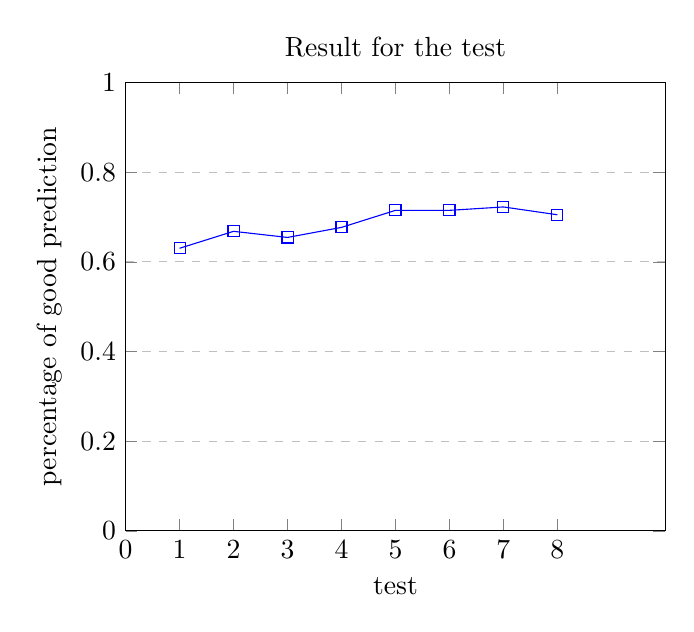
\begin{tikzpicture}
\begin{axis}[
    title={Result for the test},
    xlabel={test },
    ylabel={percentage of good prediction},
    xmin=0, xmax=10,
    ymin=0, ymax=1,
    xtick={0,1,2,3,4,5,6,7,8},
    ytick={0,0.2,0.4,0.6,0.8,1},
    legend pos=north west,
    ymajorgrids=true,
    grid style=dashed,
]
 
\addplot[
    color=blue,
    mark=square,
    ]
    coordinates {
    (1,0.6302)(2,0.66800)(3,0.65440)(4,0.67680)(5,0.71480)(6,0.71480)(7,0.72240)(8,0.70500)
    };
 
\end{axis}
\end{tikzpicture} \\
We can see that the best way I found is the way I describe it in the base with 8 dictionnaries for four different threshold and and a length of the word study which from 1 or 2.

\end{document}